\documentclass[a4paper, 14pt]{extarticle}
\usepackage[russian]{babel}
\usepackage[T1]{fontenc}
\usepackage{fontspec}
\usepackage{indentfirst}
\usepackage{enumitem}
\usepackage{graphicx}
\usepackage[
  left=20mm,
  right=10mm,
  top=20mm,
  bottom=20mm
]{geometry}
\usepackage{parskip}
\usepackage{titlesec}
\usepackage{xurl}
\usepackage{hyperref}
\usepackage{float}
\usepackage[
  figurename=Рисунок,
  labelsep=endash,
]{caption}
\usepackage[outputdir=build, newfloat]{minted}

\hypersetup{
  colorlinks=true,
  linkcolor=black,
  filecolor=blue,
  urlcolor=blue,
}

\renewcommand*{\labelitemi}{---}
\setmainfont{Times New Roman}
\setmonofont{JetBrains Mono}[
  SizeFeatures={Size=11},
]

\newenvironment{code}{\captionsetup{type=listing}}{}
\SetupFloatingEnvironment{listing}{name=Листинг}

\setminted{
  fontsize=\footnotesize,
  frame=lines,
  framesep=2mm,
}

\setlength{\parskip}{6pt}

\setlength{\parindent}{1cm}
\setlist[itemize]{itemsep=0em,topsep=0em,parsep=0em,partopsep=0em,leftmargin=2.0cm,wide}
\setlist[enumerate]{itemsep=0em,topsep=0em,parsep=0em,partopsep=0em,leftmargin=2.0cm,wide}

\renewcommand{\thesection}{\arabic{section}.}
\renewcommand{\thesubsection}{\thesection\arabic{subsection}.}
\renewcommand{\thesubsubsection}{\thesubsection\arabic{subsubsection}.}

\titleformat{\section}{\normalfont\bfseries}{\thesection}{0.5em}{}
\titleformat{\subsection}{\normalfont\bfseries}{\thesubsection}{0.5em}{}

\titleformat*{\section}{\normalfont\bfseries}
\titleformat*{\subsection}{\normalfont\bfseries}

\linespread{1.5}
\renewcommand{\baselinestretch}{1.5}

\begin{document}

\begin{titlepage}
  \vspace{0pt plus2fill}
  \noindent

  \vspace{0pt plus6fill}
  \begin{center}
    Санкт-Петербургский национальный исследовательский университет
    информационных технологий, механики и оптики

    \vspace{0pt plus3fill}

    Факультет инфокоммуникационных технологий

    Направление подготовки 11.03.02

    \vspace{0pt plus2fill}

    Лабораторная работа №5

    <<Создание карты изображений в HTML>>

  \end{center}

  \vspace{0pt plus9fill}
  \begin{flushright}
    Выполнил: \\
    Швалов Даниил Андреевич

    Группа: К33211

    Проверила: \\
    Марченко Елена Вадимовна
  \end{flushright}

  \vspace{0pt plus2fill}
  \begin{center}
    Санкт-Петербург

    2023
  \end{center}
\end{titlepage}

\section{Введение}

\textbf{Цель работы}: используя страницы ранее созданного web-сайта создать
карту изображений и разместить ее на одной из страниц сайта.

\section{Ход работы}

В данной лабораторной работе необходимо создать карту изображений, которая
должна поддерживать не менее 5 областей разной формы. При кликах на различные
области данного изображения выполняются разные действия. В качестве областей
были выбраны следующие страницы, на которые будет вести карта изображений:
\begin{itemize}
  \item страница входа в аккаунт;
  \item страница с котиками;
  \item страница оформления заказа;
  \item страница с информацией о компании;
  \item страница с контактами.
\end{itemize}
Первая и третья страница были взяты из лабораторной работы №4. Так как
необходимо не менее 5 областей разной формы, были добавлены еще три страницы
(страница с котиками, информации о компании и контактами).

На рис. \ref{fig:index} изображена главная страница сайта, на которой размещена
карта изображений. На ней доступен переход ко всем страницам, которые были
описаны выше. Исходный код страницы находится в приложении \ref{app:index.html}.

Карта изображений была реализована с помощью тегов \texttt{map} и \texttt{area}.
С помощью тега \texttt{map} создается сама карта изображений, а с помощью тегов
\texttt{area} указываются области изображения, которые выступают в качестве
ссылок. Для указания браузеру, что изображение является картой, был использовал
атрибут \texttt{usemap} в теге \texttt{img}. Для создания областей
использовались различные типы фигур: \texttt{rect}, \texttt{shape} и
\texttt{poly}.

\begin{figure}[H]
  \centering
  \fbox{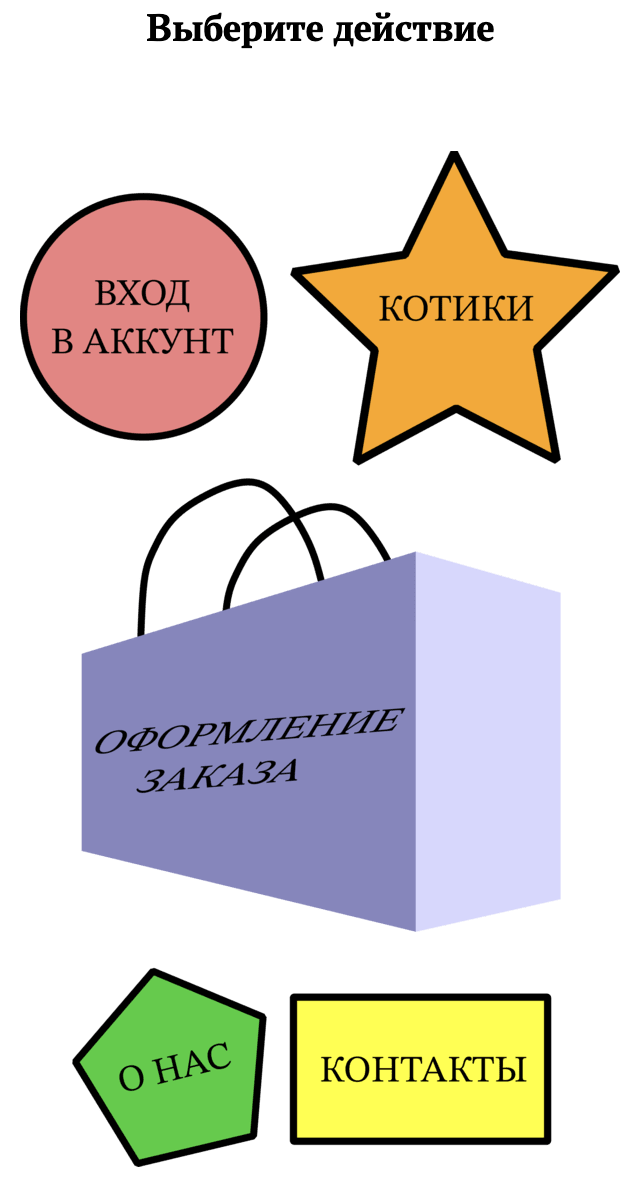
\includegraphics[width=0.4\textwidth]{images/index.png}}
  \caption{Главная страница сайта}
  \label{fig:index}
\end{figure}

При нажатии на область <<Котики>> пользователь попадает на страницу,
изображенную на рис. \ref{fig:cats}. Страница с котиками позволяет пользователю,
который чувствует стресс или усталость, получить немного позитивных эмоций.
Такой подход благотворительно сказывается на отношении пользователя к сайту, он
чувствует, что владельцы сайта заботятся о нем. Также такой ход имеет и
маркетинговые цели: человек, который увидит такую страницу на сайте, не
относящимся к котам, скорее всего, захочет поделиться таким наблюдением со
своими знакомыми и друзьями. В добавок ко всему, человеческая память очень
хорошо запоминает моменты, которые вызывают какие-либо эмоции. Таким образом,
страница с котиками позволяет сайту компании отпечататься в памяти пользователя.
Исходный код страницы расположен в приложении \ref{app:cats.html}.

\begin{figure}[H]
  \centering
  \fbox{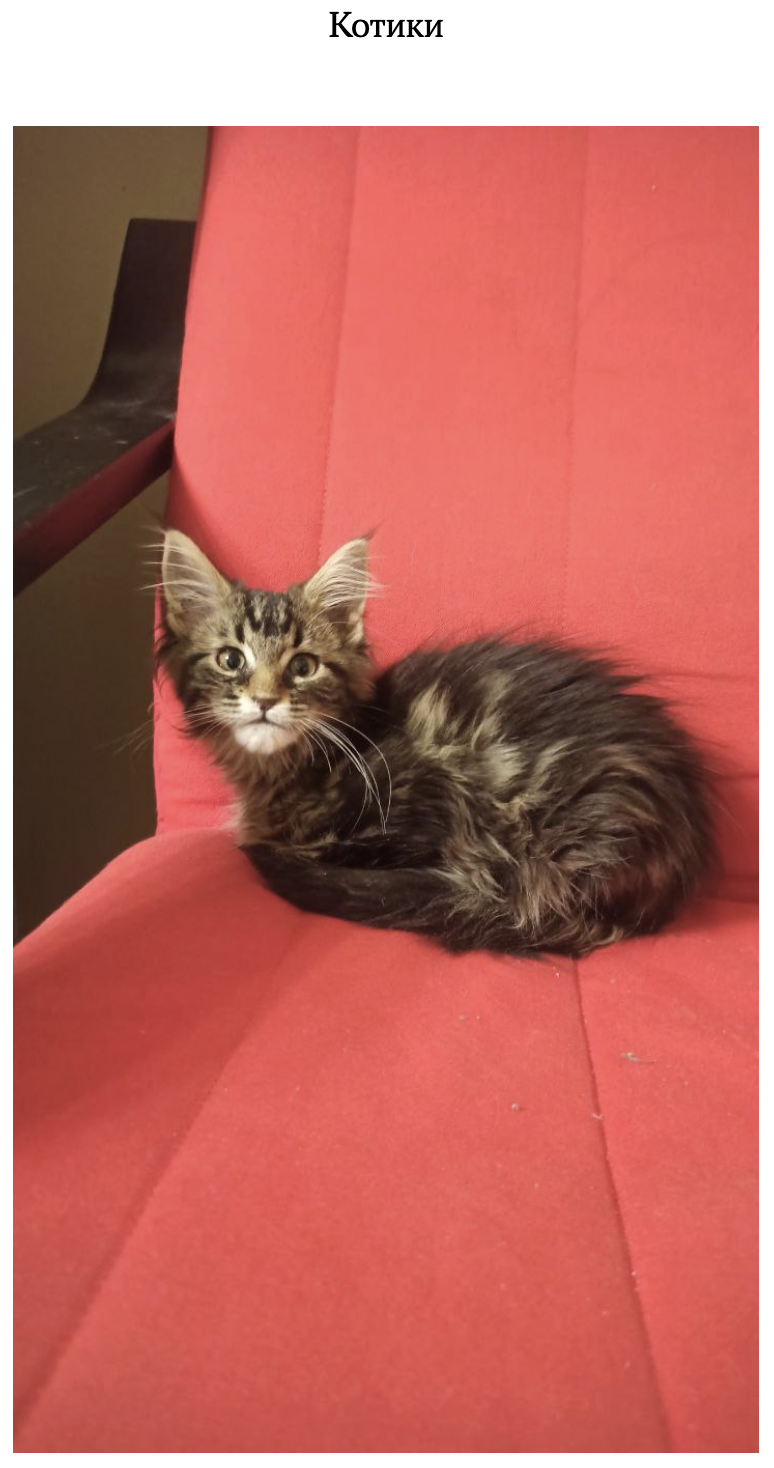
\includegraphics[width=0.4\textwidth]{images/cats.png}}
  \caption{Страница с котиками}
  \label{fig:cats}
\end{figure}

При нажатии на область <<О нас>> пользователь попадает на страницу с информацией
о компании (рис. \ref{fig:about}), которая позволяет больше узнать о
деятельности компании. Это помогает компании укрепить доверие пользователя к
сайту. Исходный код страницы находится в приложении \ref{app:about.html}.

\begin{figure}[H]
  \centering
  \fbox{
\includegraphics[width=\textwidth]{images/about.png}}
  \caption{Страница с информацией о компании}
  \label{fig:about}
\end{figure}

При нажатии на область <<Контакты>> открывается страница с контактами (рис.
\ref{fig:contacts}). Она будет полезна пользователю в том, случае, если у него
возникнет потребность связаться с владельцами сайта. Исходный код страницы
находится в приложении \ref{app:contacts.html}.

\begin{figure}[H]
  \centering
  \fbox{
\includegraphics[width=\textwidth]{images/contacts.png}}
  \caption{Страница с контактами}
  \label{fig:contacts}
\end{figure}

\section{Вывод}

В ходе выполнения лабораторной работы я, используя страницы ранее созданного
web-сайта, создал карту изображений и разместил ее на одной из страниц сайта.

\newpage

\appendix

\titleformat{\section}[display]
{\normalfont\bfseries}
{\centering Приложение\ \thesection}
{0pt}{\centering}
\renewcommand{\thesection}{\Asbuk{section}}

\section{Исходный код главной страницы}
\label{app:index.html}

\begin{code}
  \inputminted{html}{../task-1/index.html}
\end{code}

\newpage

\section{Исходный код страницы входа в аккаунт}
\label{app:login.html}

\begin{code}
  \inputminted{html}{../task-1/login.html}
\end{code}

\newpage

\section{Исходный код страницы успешного входа в аккаунт}
\label{app:login-success.html}

\begin{code}
  \inputminted{html}{../task-1/login-success.html}
\end{code}

\newpage

\section{Исходный код страницы оформления заказа}
\label{app:order.html}

\begin{code}
  \inputminted{html}{../task-1/order.html}
\end{code}

\newpage

\section{Исходный код страницы успешного оформления заказа}
\label{app:order-success.html}

\begin{code}
  \inputminted{html}{../task-1/order-success.html}
\end{code}

\newpage

\section{Исходный код страницы с котиками}
\label{app:cats.html}

\begin{code}
  \inputminted{html}{../task-1/cats.html}
\end{code}

\newpage

\section{Исходный код страницы с информацией о компании}
\label{app:about.html}

\begin{code}
  \inputminted{html}{../task-1/about.html}
\end{code}

\newpage

\section{Исходный код страницы с контактами}
\label{app:contacts.html}

\begin{code}
  \inputminted{html}{../task-1/contacts.html}
\end{code}

\newpage

\section{Исходный код стилей}
\label{app:style.css}

\begin{code}
  \inputminted{css}{../task-1/css/style.css}
\end{code}

\newpage

\section{Исходный код скрипта работы с БД}
\label{app:database.php}

\begin{code}
  \inputminted{php}{../task-1/database.php}
\end{code}

\newpage

\section{Исходный код скрипта входа в аккаунт}
\label{app:login.php}

\begin{code}
  \inputminted{php}{../task-1/login.php}
\end{code}

\newpage

\section{Исходный код скрипта оформления заказа}
\label{app:order.php}

\begin{code}
  \inputminted{php}{../task-1/order.php}
\end{code}


\end{document}
